\section{Exercice 9}
\subsection{Question 1}

\begin{center}
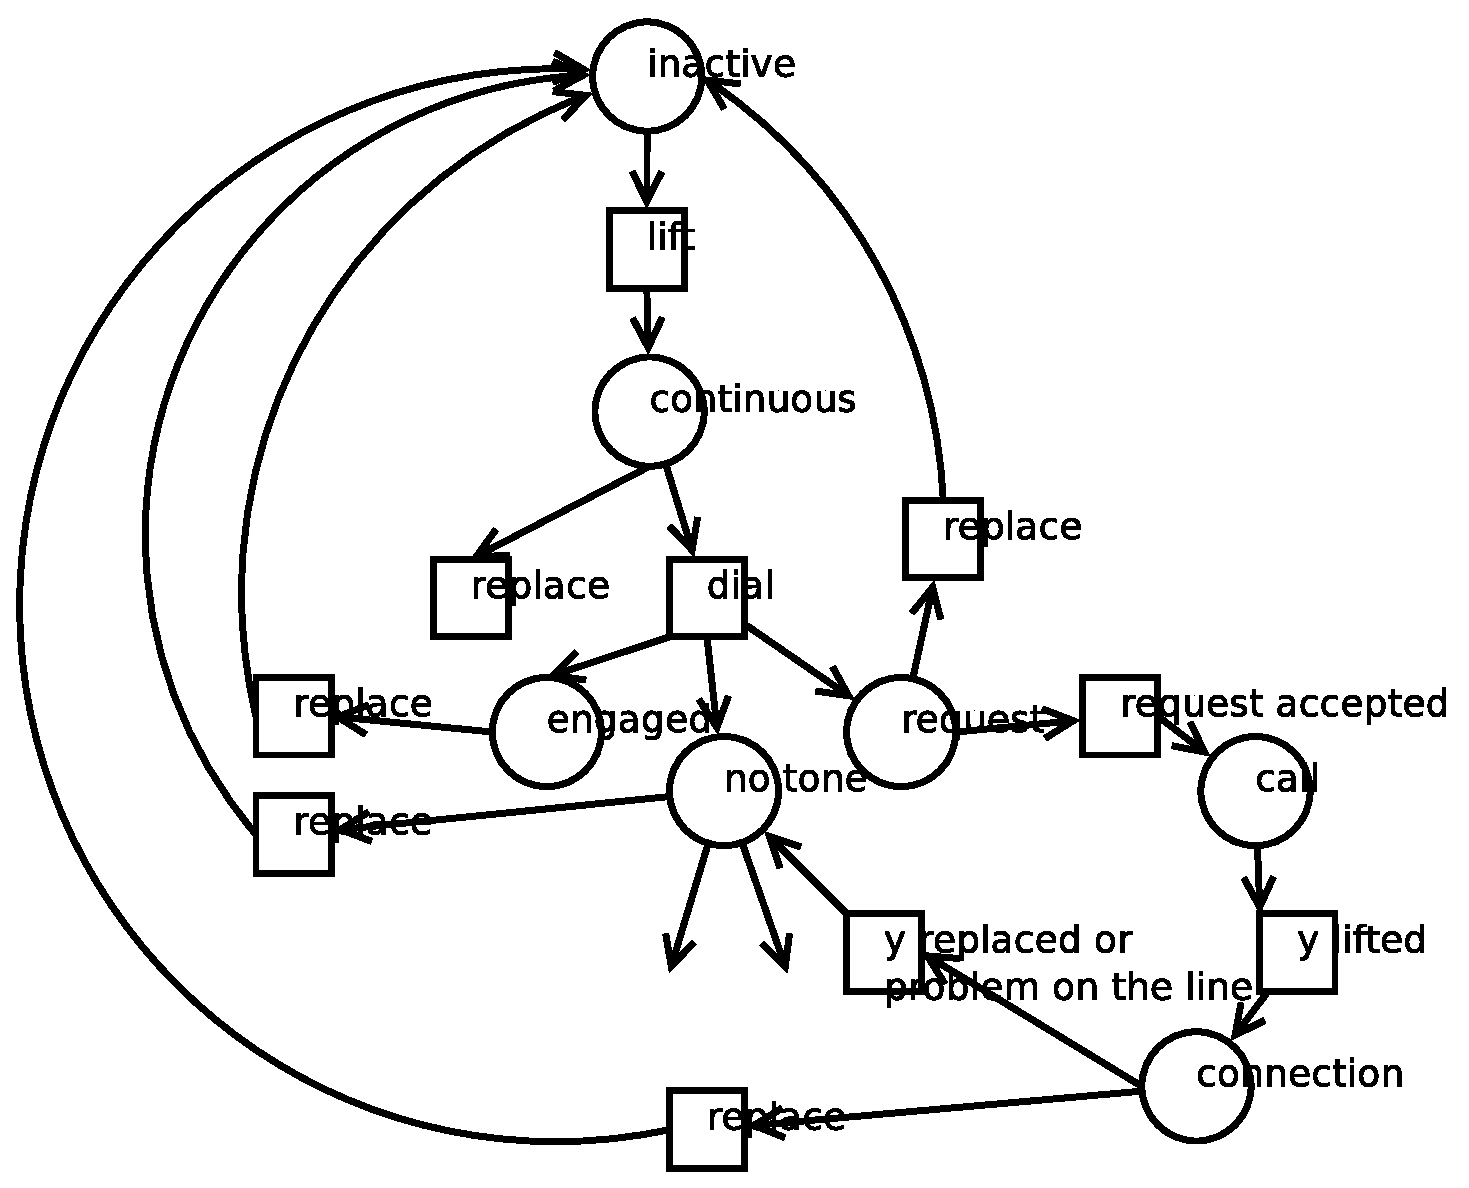
\includegraphics[height = 8cm]{exo9_1.eps}
\end{center}

\subsection{Question 2}

TODO : simulation TIna

Quand un téléphone appelle son propre numéro, il tombe directement dans l'état \textbf{engaged}.

Le téléphone appelé peut mettre fin à la conversation, le téléphone
appelant tombe alors dans l'état \textbf{no tone}.

Ce modèle est effectif en France, mais il demeure basique : un certain
nombre de fonctionnalités <<~modernes~>> manquent à l'appel. Ainsi,
c'est le cas du rappel automatique en cas de correspondant occupé, ou
de la mise en attente.

\subsection{Question 3}

Pour représenter le caractère activé ou désactivé d'un numéro de
téléphone, nous proposons de rajouter deux couleurs \textit{activé}
$a$ et \textit{désactivé} $d$.

Le modèle correspondant est le suivant~:

+ faire le schéma

\begin{center}
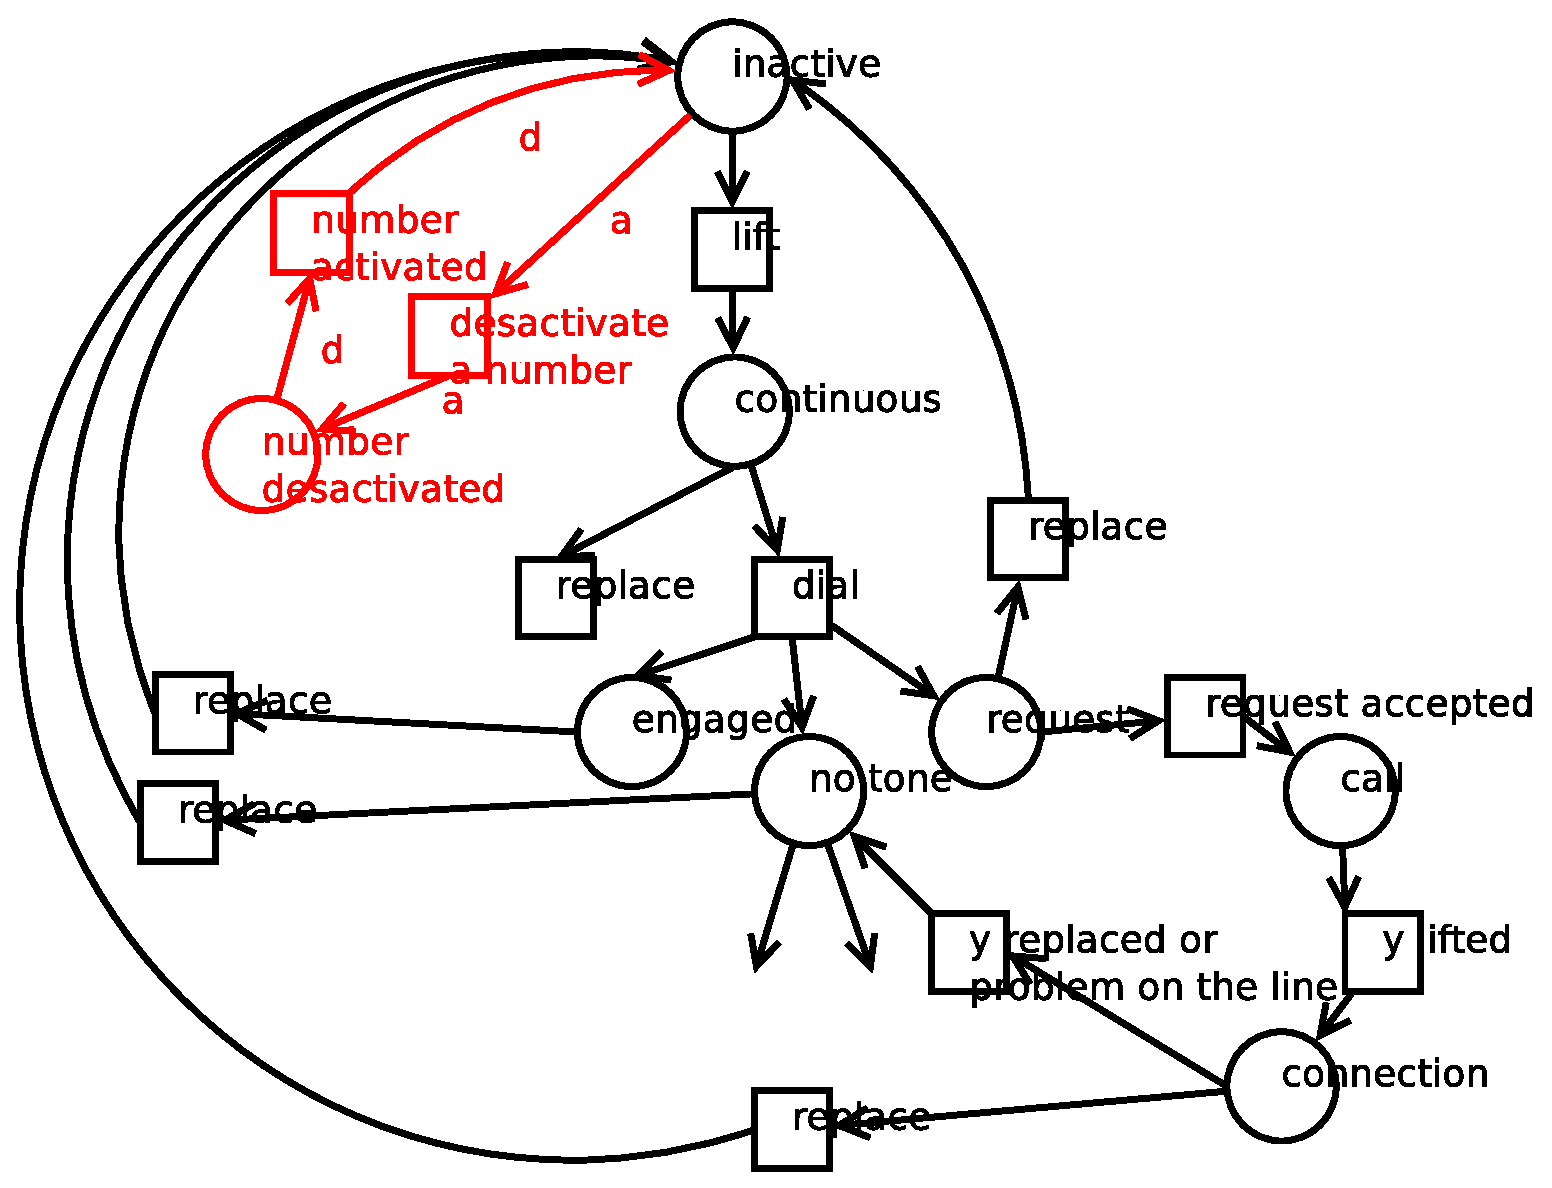
\includegraphics[height = 8cm]{exo9_2.eps}
\end{center}
\subsection{Question 4}

Afin de tenir compte des dépassements de délai, on transforme le
réseau de pétri en réseau de pétri temporisé de la manière suivante~:

+ faire le schéma

\begin{center}
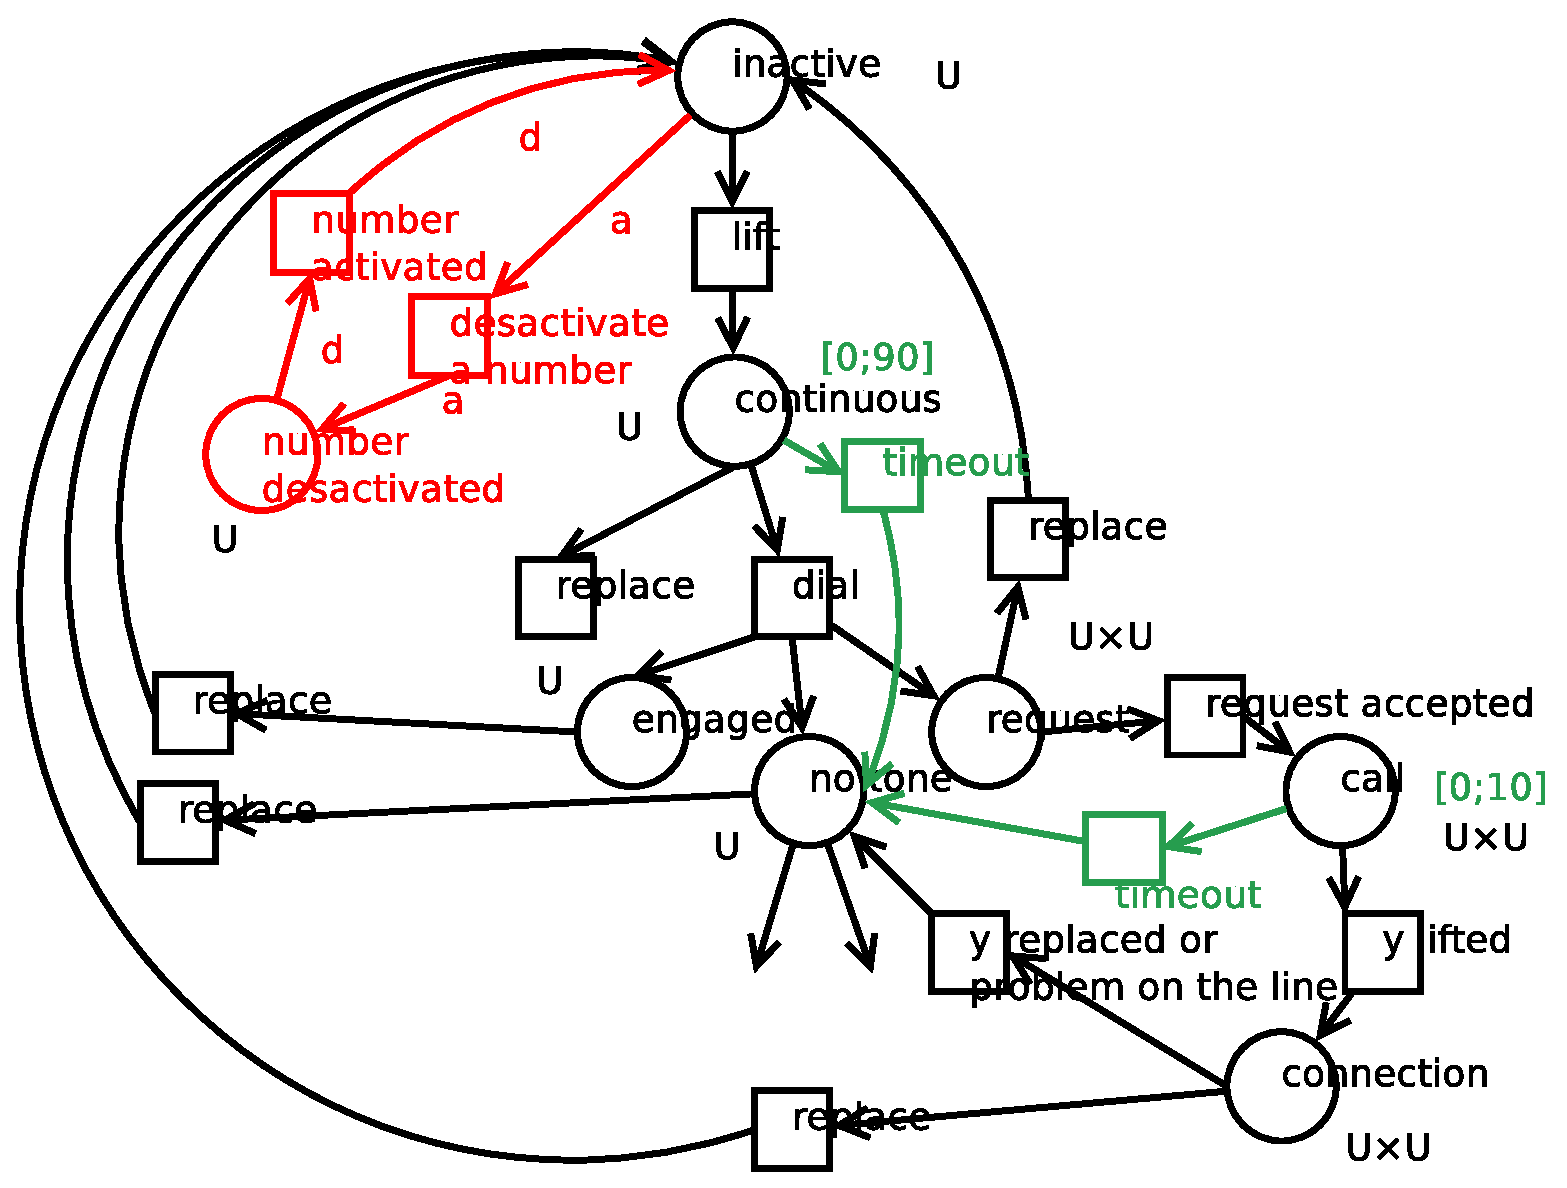
\includegraphics[height = 8cm]{exo9_3.eps}
\end{center}
